\section{Zusammenfassung}
Rot heißt klausurrelevant

\subsection{Themenübersicht}
Die Themenübersicht ist temporär bis sich das in halts verzeichnis selbst erzeugt
\begin{itemize}
    \item Wahrscheinlichkeitsräume Wahrscheinlichkeitsverteilung, Laplace-Modell Satz 3.2
    \item Kombinatorik
    \begin{itemize}
        \item Multiplikationsregel
        \item Summenregel
        \item k-Permutation \& k-Kombination mit / ohne Wiederholung
    \end{itemize}
    \item Zähldichte
    \item Wichtige diskrete Verteilungen
    \begin{itemize}
        \item Binomialvertelung
        \item Poission-Verteilung
    \end{itemize}
    \item Wichtige stetige Verteilungen
    \begin{itemize}
        \item Exponential-Verteilung
        \item Normalverteilung
    \end{itemize}
    \item Übergangswahrscheinlichkeiten und bedingte Wahrscheinlichkeitsverteilung
    \begin{itemize}
        \item Bedingte Wahrscheinlichkeits
        \item Formel von der totalen Wahrscheinlichkeit
        \item Formel von Bayes
    \end{itemize}
    \item Maßzahlen von Verteilungen
    \begin{itemize}
        \item Erwartungswert
        \item Varianz
        \item Standardabweichung Satz 12.3 Satz 12.7
    \end{itemize}
    \item Parameterschätzung Konfidenzintervall
\end{itemize}

\subsection{Deskriptive Statistik (Wahrscheinlichkeitstheorie)}

Gegeben sei die Stichprobe $x=(x_1,..,x_n)$ vom Umfang $n$ mit Werten in $\mathbb{R}$.
\[\overline{x}:= \frac{1}{n}*\sum_{i = 1}^{n}=\frac{x_1+...+x_n}{n}     \]

heißt Stichproben-Mittel,

\[{s_x}^2:=\frac{1}{n-1}\sum_{i=1}^{n}(x_i-\overline{x})^2   =\frac{(x_1-\overline{x})^2+...+(x_n-\overline{x})^2}{n-1}\]

Stichproben-Varianz, wobei $n\geq 2$

\[s_x := +\sqrt{{s_x}^2} \]

Stichproben-Standaedabweichung und

\[v_x := \frac{s_x}{x} \]

für $x_1,...,x_n >0 $ heißt Stichproben-Variantionskoeffizient.\\

Der Stichproben-Median (Zentralwert) von $x$

\[\tilde{x} :=\begin{cases}x_{(\frac{n+1}{2})}\textrm{    ,falls $n$ ungerade}\\
    \frac{1}{2}*(x_{(\frac{n}{2})}+x_{(\frac{n}{2}+1)})\textrm{ ,falls n gerade}\end{cases}\]

Stichproben -$\alpha$-Quantil\\

Sei $\alpha \in (0,1)$ und $k:=[n*\alpha]$. Dann heißt

\[\tilde{x}_\alpha  :=\begin{cases}x_{(k+1)}\textrm{,falls $n*\alpha \notin \mathbb{N} $}\\
    \frac{1}{2}*(x_{(k)}+x_{(k+1)})\textrm{,sonst}\end{cases}\]


$\alpha$-getrimmte Stichproben-Mittel(kommt nicht dran)\\

Sei $\alpha \in [0,0.5]$ und $k:=[n*\alpha ]$. Dann heißt

\[\tilde{x}_\alpha := \frac{1}{n-2*k}*(x_{(k+1)}+...+x_{(n-k)}) \]

das $\alpha $-getrimmte (gestutzte) Stichproben-Mittel.


\subsection{Wahrscheinlichkeitsräume}

auch Stochastisches Modell Zufallsexperiment\\
ist ein Tripel($\Omega ,\mathcal{E}, \mathbb{P}$)
\begin{itemize}
    \item [i] Grundraum $\Omega\neq \varnothing  $
    \item [ii] Ereignisraum $\varepsilon $
    \item [iii] Wahrscheinlichkeitsmaß $\mathbb{P}$
\end{itemize}
$\mathbb{P} :\varepsilon \longleftarrow [0,1]$ weißt jedem Ereignis eine Wahrscheinlichkeit zu.\\

Wie berechent man das Wahrscheinlichkeitsmaß?\\
\renewcommand{\labelenumi}{\alph{enumi})}
\begin{enumerate}
    \item $\mathbb{P}(\emptyset) = 0$
    \item $\mathbb{P} (\sum_{j = 1}^{n} A_j)=\sum_{j = 1}^{n}\mathbb{P} (A_j) $ ,falls $A_1,...,A_n$ paarweise disjunkt (endliche Additivität)
    \item $\mathbb{P} (A^c)= 1-\mathbb{P} (A)$, $\forall A:A\in \mathcal{A} \longleftarrow A^c\in \mathcal{A} $
    \item $A\subset B \longleftarrow \mathbb{P}(A)\leq \mathbb{P} (B)$(Monotonie)
    \item $\mathbb{P} (A\cup B)=\mathbb{P} (A)+\mathbb{P} (B)-\mathbb{P} (A\cap B)$
\end{enumerate}
c) Wegen $\Omega = A+A^c$ und b) gilt $1 = \mathbb{P} (\Omega)=\mathbb{P} (A)+\mathbb{P} (A^c)$.

genauers wird in den Späteren Vorlesung erläutert.\\

\section{Kombinatorik}
Erscheint ein Laplace-Modell in einer Situation angemessen, so ist die Wahrscheinlichkeit eines Ereignisses $A$

\[P(A)=\frac{\textrm{Anzal der für $A$ \dq günstigen \dq Fälle}}{\textrm{Anzal aller mölicen Fälle}} \]

Die Lere vom systematischen Abzlen endlicher \dq strukturierter \dq Mengen heißt Kombinatorik.

\subsection{Multiplikationsregel (Produktregel)}

\[m_1\cdot m_2 \cdot ... \cdot m_k\]

Beispiele: Wie viele Möglichkeiten ggibt es jeweils?\\

\begin{itemize}
    \item Auf der Speisekarte stehen 3 Vorspeisen, 10 Hauptgerichte und 2 Desserts. Wie viele 3-gängige Menüs kann man zusammenstellen? $\Longrightarrow 3\cdot 10\cdot 2 = 60$
    \item Ein roter und ein blauer Würfel werden geworfen.$\Longrightarrow 6\cdot 6=36$
    \item Bei einem Neuwagen gibt es 8 aufpriespflichtige Zusatzoptionen, die in beliebiger Kombination zu- oder abbestellt werden können.$\Longrightarrow 2\cdot 2\cdot ...\cdot 2 = 2^8=256$
\end{itemize}

Wenn es Experminente sind in denen zurückgelegt wird kann die \texttt{Produktregel nicht angewendet} werden, da Werte nicht beliebig kombinierbar sind.


\subsection{Summenregel}

Wenn es mehrere Gruppen mit $m_1$ bzw. $...m_n$ verschiedenen Werte gibt, die sich gegenseitig ausschließen, dann gibt es insgesamt $m_1+...+m_n$ mögliche Werte.\\

\texttt{Beispiel}\\
Auf der Speisekarte sind als Hauptspeise 10 Fleischgerichte, 4 Fischgerichte und 2 vegetarische Gerichte zur Auswahl. Zusätzlich gibt es 3 Vorspeisen und 5 Desserts zur Auswahl. Wie viele 3 gängige Menüs kann man zusammenstellen?

\[3\cdot (10+4+2)\cdot 5=240\]

\subsection{Permutation u. Kombinationen}

Tabelle wird nachgereicht solbald internet\\

Hier ist:

\begin{align}
    \binom{m}{l}&:=\frac{m!}{l!\cdot (m-l)!} (m,l\in\mathbb{N}_0,l\leq m)\\
    0!&=1\\
    m!&=1\cdot 2\cdot ...\cdot m.\\
    n^{\underline{k}}&=\frac{n!}{(n-k)!}.  
\end{align}

k-Permutation aus M ohne Wiederholung

\[\Longrightarrow \left\lvert \Omega \right\rvert = \frac{n!}{(n-k!)}=\binom{n}{k}k!\]

\[\left[ \binom{n}{k}=\frac{n!}{k!(n-k)!}\right]\]

k-Kombination aus M ohne Wiederholung

\[\Longrightarrow \left\lvert \Omega \right\rvert = \frac{n!}{k!(n-k!)}=\binom{n}{k}\]

k-Kombination aus M mit Wiederholung

\[\Longrightarrow \left\lvert \Omega \right\rvert = \binom{n+k-1}{k}\]


\begin{table}[ht]
    \begin{tabular}{|l|l|l|l|}
    \hline
    \textbf{Wdh?} & \textbf{Rhf?} & \textbf{Anzahl. Möglichkeiten} & \textbf{Beispiel} \\ \hline
    mit\footnote[1]{Mehrmals die gleiche Wahhl treffen (\textbf{mit Wdh.})}           & mit\footnote[3]{Es ist wichtig, in welcher Reihenfolge wie endschieden wurde(\textbf{mit Reihenf.})}           & $n^k$                        & $k$ Personen werfen je einen Würfel(also $n=6$)           \\ \hline
    ohne\footnote[2]{Jedes Mal eine andere Wahl treffen muss(\textbf{o. Wdh.})}         & mit\footnotemark[3]          & $n!$                    & Auf wie vielen Arten lassen sich $n$ Objekte sortieren?     \\ \hline
    ohne\footnotemark[2]         & mit\footnotemark[3]           & $\frac{n!}{(n-k)!} $                    & \begin{tabular}[c]{@{}l@{}}Lotto  \dq$k$ aus $n$\dq mit Ziehungs-Reihenfolge\\.\end{tabular}            \\ \hline
    ohne\footnotemark[2]         & ohne\footnote[4]{Es ist nur wichtig, wie oft welche Entscheidung getroffen wurde.\textbf{o. Reihenf.}}          & $\binom{n}{k}=\frac{n!}{k!\cdot(n-k)!} $                         & \begin{tabular}[c]{@{}l@{}}Normales Lotto \dq$k$ aus $n$\dq \\.\end{tabular}          \\ \hline
    mit\footnotemark[1]           & ohne\footnotemark[4]          &  $\binom{n+k-1}{k}$                               &  \begin{tabular}[c]{@{}l@{}}$k$ nicht unterscheidbare Würfel\\ werden in einem Würfelbecher geworfen  \end{tabular}        \\ \hline
    \end{tabular}
    \caption{Wann muss welche Formel angewendet werden?}
    \label{tab:my-table}
    \end{table}

\newpage

\section{Zufallsgröße und Wahrscheinlichkeitsverteilung}
Muss sich seperrat angeschaut werden script unbrauchbar.
\begin{align}
    x &=\textrm{sei ...}&  x&=x_i & P(X=x_i)
\end{align}
$\longrightarrow$ Würfel $2\times $ werfen, 6 oder keine 6\\
$\longrightarrow$ $2\times 6$ 10€ Gewinn $2\times \overline{6}$ 0€ Gewinn sonst 5€ Gewinn.\\

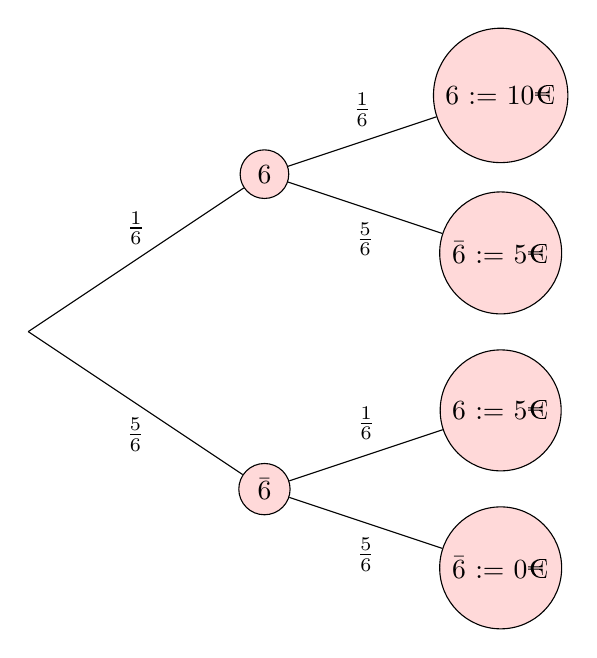
\begin{tikzpicture}[
    circ/.style={draw=black,fill=red!15,circle},
    grow=right,
    level 1/.style={sibling distance=4cm},
    level 2/.style={sibling distance=2cm},
    level distance=3cm]
 \node [coordinate] {}
   child {
     node[circ] {$\bar{6}$}
       child { node[circ] {$\bar{6}$ := 0€}
         edge from parent
         node [below=2] {$\frac{5}{6} $}}
       child { node[circ] {$6$ := 5€}
         edge from parent
         node [above=2] {$\frac{1}{6}$}}
     edge from parent
     node [below=2] {$\frac{5}{6}$}
     }
   child {
     node[circ] {$6$}
       child { node[circ] {$\bar{6}$ := 5€}
         edge from parent
         node [below=2] {$\frac{5}{6}$}}
       child { node[circ] {$6$ := 10€}
         edge from parent
         node [above=2] {$\frac{1}{6}$}
   }
    edge from parent
    node [above=2] {$\frac{1}{6}$}
   };
 \end{tikzpicture}

 \begin{table}[ht]
    \begin{tabular}{llll}
    \textbf{}                       & $x_1$ & $x_2$      & $x_3$ \\
    \multicolumn{1}{l|}{$x=x_i$}    & 10    & 5          & 0     \\ \hline
    \multicolumn{1}{l|}{$P(x=x_i)$} & $\frac{1}{36}$       & $\frac{10}{36} $ & $\frac{25}{36} $     
    \end{tabular}
    \caption{}
    \label{tab:my-table}
    \end{table}

\subsection{Zähldichte}

Muss sich seperrat angeschaut werden script unbrauchbar.

\[f_x(t)=P(X=t)\]

\section{Wichtige diskrete Verteilungen}

\subsection{Binomialverteilung}

Seien $n$ eine natürliche Zahl und $0\leq p\leq 1$. Die zur Zähldichte

\[k\longrightarrow f(k)=\binom{n}{k}\cdot p^k\cdot (1-p)^{n-k},k=0,...,n, \]

gehörende Verteilung heißt \texttt{Binomialverteilung} mit den Parametern $n$ und $p$ und wird mit $Bin(n,p)$ bezeichnet.

\subsection{Poisson-Verteilung}

Ideales Zufallsexperiment mit kleiner Erfolgswahrscheinlichkeit $p$ werde $n$ mal in unabhängiger Folge durchführt ($n$ groß). Ist $X$ die zufällige Anzahl von Treffern, so gilt mit $\lambda := n\cdot p$ näherungsweise

\[\mathbb{P} (X=k) = \binom{n}{k}\cdot p^k \cdot (1-p)^{n-k}\thickapprox e^{-\lambda}\cdot \frac{\lambda^k}{k!}  \]

für $k\leq n$.

Wann es angewendet wird muss sic noc anescaut werden.

\section{Wichtige stetige Verteilung}

\subsection{Normalverteilung}

\[P(X\leq x)= F(x)=\Phi_{\mu ,\sigma ^2}(x)=\int_{x}^{-\infty} \frac{1}{\sigma\sqrt{2\pi}}\cdot 2^{-(x-\mu)^2/(2\sigma^2)} \,dx \]

Die Verteilungsfunktion $\Phi_{\mu ,\sigma ^2}(x)$ der Normalverteilung ist \textbf{nicht als geschlossene Funktion} darstellbar(d.h. ohne Integral oder unendliche Reihe). Für die Standardnormalverteilung ist sie tabelliert.

\[\Phi(-x)=1-\Phi(x)\]
Sei $X~\mathcal{N} (\mu,\sigma^2)$. Dann gilt

\[\mathbb{P} (X\leq t)=\Phi_{\mu ,\sigma ^2}(t)=\Phi\left( \frac{t-\mu}{\sigma} \right)\]

Beispiel: Sei$X~\mathcal{N} (2,9)$. Dann ist

\begin{align}
    P(1\leq X\leq 4)&=F_X(4)-F_X(1)\\
    &=\Phi\left(\frac{4-2}{\sqrt{9}}\right)-\Phi\left(\frac{1-2}{\sqrt{9} } \right)\\
    &=\Phi(0.67)-\Phi(-0.33)\\
    &=0.7486-(1-\Phi(0.33))\\
    &=0.7486-(1-0.6293)\\
    &=0.3779
\end{align}

Beispiel: Angenommen das Gewicht G der Studenten der DHBW Karlsruhe sei normalverteilt mit $\mu =75$kg und $\sigma=5$kg.\\

Bestimmen sie $P(69kg<G<81kg)$ rechnerisch mittels Tabelle.

\[P(69kg<G<81kg)=\Phi_{75,5^2}(81)-\Phi_{75,5^2}(69)\]

Zwei Studenten werden zufällig und unabhängig voneinander ausgewählt. Wie wahrscheinlich ist es das beide zwischen 69 und 81kg wiegen?
\begin{align}
    P(A)=P(B)&=76.9\%\textrm{ Ergebnis aus vorheriger Aufgabe}\\
    P(A\cap B)=P(A)\cdot P(B)&=0.769^2\thickapprox \underline{59.1\% }
\end{align}


\subsection{Exponential Verteilung}

Sollte in der 6 Vorlesung sein habe ich aber noch nicht gefunden.

\section{Übergangswahrscheinlichkeiten und bedingte Wahrscheinlichkeiten}